\subsection{离散傅里叶变换}

离散时间信号的傅里叶频谱是连续的,而计算机只能处理离散的数据,
因此需要将连续的频谱离散化,这就是离散傅里叶变换。

\subsubsection{离散傅里叶变换的定义}

\begin{definition}
    由长度为 $L$ 的序列 $x(n), n = 0, 1, \cdots, L - 1$,
    求其 DTFT 谱上 $[0, 2\pi]$ 区间上均匀分布的 $N$ 个谱值
    \begin{align*}
        \omega_k = \frac{2\pi k}{N}, \quad k = 0, 1, \cdots, N - 1,
    \end{align*}
    的过程称为\bd{离散傅里叶变换}(DFT),记为
    \begin{align*}
        X'(\omega_k) = \sum_{n = 0}^{L - 1}x(n)\mathe^{-\mathi\omega_k n}.
    \end{align*}
    将其写为 $k$ 的函数形式,即
    \begin{align*}
        X(k) = \sum_{n = 0}^{L - 1}x(n)\mathe^{-2\pi\mathi k n/N}.
    \end{align*}
    记 $W_N = \mathe^{-2\pi\mathi/N}$,则
    \begin{align*}
        X(k) = \sum_{n = 0}^{L - 1}x(n)W_N^{kn},
    \end{align*}
    其中 $k = 0, 1, \cdots, N - 1$。
\end{definition}

\begin{exercise}
    利用 DFT 的公式计算
    \begin{align*}
        x(n) = \sin(\frac{2\pi}{N}mn)
    \end{align*}
    的 $N$ 点 DFT,其中 $0 \le n \le N - 1, 0 < m < N$ 且 $m \in \set{Z}$。
\end{exercise}

\begin{solution}
    由于 $\sin\theta = (\mathe^{\mathi\theta} - \mathe^{-\mathi\theta})/(2\mathi)$,因此
    \begin{align*}
        x(n) & = \sin\left(\frac{2\pi}{N}mn\right) \\
        & = \frac{\mathe^{2\pi\mathi mn/N} - \mathe^{-2\pi\mathi mn/N}}{2\mathi} \\
        & = \frac{\mathi}{2} \left(W_N^{mn} - W_N^{-mn}\right).
    \end{align*}
    由 DFT 的定义可知
    \begin{align*}
        X(k) & = \sum_{n = 0}^{N - 1} x(n)W_N^{kn} \\
        & = \sum_{n = 0}^{N - 1} \sin\left(\frac{2\pi}{N}mn\right)W_N^{kn} \\
        & = \frac{\mathi}{2}\sum_{n = 0}^{N - 1}\left(W_N^{mn} - W_N^{-mn}\right)W_N^{kn} \\
        & = \frac{\mathi}{2}\sum_{n = 0}^{N - 1}W_N^{(k + m)n} - \frac{\mathi}{2}\sum_{n = 0}^{N - 1}W_N^{(k - m)n} \\
        & = \frac{\mathi}{2} \cdot \frac{1 - W_N^{(k + m)N}}{1 - W_N^{k + m}} - \frac{\mathi}{2}\sum_{n = 0}^{N - 1}\left(W_N^{k - m}\right)^n \\
        & = 0 - \frac{\mathi}{2}\sum_{n = 0}^{N - 1}\left(W_N^{k - m}\right)^n \\
        & = -\frac{\mathi}{2}\sum_{n = 0}^{N - 1}\left(W_N^{k - m}\right)^n.
    \end{align*}
    当 $k = m$ 时,$X(k) = -\mathi N/2$;当 $k \ne m$ 时,$X(k)$ 为等比数列求和,故
    \begin{align*}
        X(k) & = \frac{\mathi}{2} \cdot \frac{1 - \left(W_N^{k - m}\right)^N}{1 - W_N^{k - m}} \\
        & = 0.
    \end{align*}
    综上所述,
    \begin{align*}
        X(k) = -\frac{\mathi N}{2}\delta(k - m).
    \end{align*}
\end{solution}

\subsubsection{DFT 的矩阵表示}

\begin{definition}[DFT 的矩阵表示]
    如果将 $x(n)$ 看作是一个列向量 $\vct{x}$,将 $X(k)$ 看作是一个列向量 $\vct{X}$,
    则 DFT 可以表示为
    \begin{align*}
        \vct{X} = \begin{bmatrix}
            X_0 \\ X_1 \\ \vdots \\ X_{N - 1}
        \end{bmatrix}
        = A \begin{bmatrix}
            x_0 \\ x_1 \\ \vdots \\ x_{L - 1}
        \end{bmatrix} = A\vct{x},
    \end{align*}
    其中 $A$ 是 DFT 的矩阵表示,即
    \begin{align*}
        A_{kn} = W_N^{kn} = \mathe^{-2\pi\mathi kn/N}.
    \end{align*}
    这是因为由 DFT 的定义,有
    \begin{align*}
        X_k = \sum_{n = 0}^{L - 1}W_N^{kn}x_n,
    \end{align*}
\end{definition}

\subsubsection{$N$ 与 $L$ 的关系}

从理论上讲,DFT 中的 $N$ 与 $L$ 之间是相互独立的。$L$ 是数据记录中
时域样本的数目,它可能是无限的;而 $N$ 则是对 DTFT 进行抽样时的频率点的数目。
通常,在讨论和使用 DFT(特别是编程实现)时常常取 $N = L$。
既然 $L$ 与 $N$ 没有什么必然的联系,那么,为什么要设它们相等?
这是出于什么考虑呢?

\begin{example}[$N > L$ 的情况]
    $N > L$ 说明频域的采样点个数 $N$ 比序列的长度 $L$ 多,
    此时只需要在序列尾部补\bd{任意数目}的 $0$ 即可。新序列的 DFT 与原序列的 DFT 结果
    相同。
\end{example}

\begin{theorem}
    设长度为 $L$ 的序列 $x(n)$ 的 DFT 为 $X(k)$,则将其补 $N - L$ 个 $0$,
    设得到的新序列为 $x_D(n)$,其 DFT 为 $X_D(k)$。用向量表示为
    \begin{align*}
        \vct{x} = \begin{bmatrix}
            x_0 \\ x_1 \\ \vdots \\ x_{L - 1}
        \end{bmatrix}, \quad
        \vct{x}_D = \begin{bmatrix}
            x_0 \\ x_1 \\ \vdots \\ x_{L - 1} \\ 0 \\ \vdots \\ 0
        \end{bmatrix}.
    \end{align*}
    此时,有
    \begin{align*}
        X_D(k) = X(k).
    \end{align*}
\end{theorem}
    
\begin{proof}
    由 DFT 的定义可知
    \begin{align*}
        X_D(k) & = \sum_{n = 0}^{N - 1}x_D(n)W_N^{kn} \\
        & = \sum_{n = 0}^{L - 1}x(n)W_N^{kn} \\
        & = X(k).
    \end{align*}
\end{proof}

\begin{definition}[回绕序列]
    设有序列 $x(n)$ 的长度为 $L$,则定义其关于 $N(N < L)$ 的\bd{回绕序列}为
    \begin{align*}
        \rev{x}(n) = \sum_{m = 0}^{+\infty}x(mN + n),
    \end{align*}
    其中 $n = 0, 1, \cdots, N - 1$。
    这类似于将长度为 $L$ 的序列切成每块长度为 $N$ 的子序列,然后将这些子序列按位相加,
    如果一块子序列的长度不足 $N$,则在末尾补 $0$。如图 \ref{fig:wrapped_sequence} 所示。
    \begin{figure}[H]
        \centering
        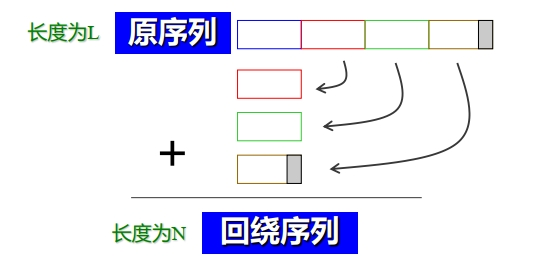
\includegraphics[width = 0.6\textwidth]{chap3/img/wrapped_sequence.png}
        \caption{回绕序列的示意图}
        \label{fig:wrapped_sequence}
    \end{figure}
\end{definition}

\begin{example}[$N < L$ 的情况]
    当 $N < L$ 时,频域的采样点个数 $N$ 少于序列的长度 $L$,此时可以将序列转为
    其回绕序列,再进行 DFT。回绕序列的 DFT 与原序列的 DFT 结果相同。
\end{example}

\begin{theorem}
    设长度为 $L$ 的序列 $x(n)$ 的 DFT 为 $X(k)$,
    其回绕序列 $\rev{x}(n)$ 的 DFT 为 $\rev{X}(k)$。
    则有
    \begin{align*}
        \rev{X}(k) = X(k).
    \end{align*}
\end{theorem}

\begin{proof}
    (方法一)
    由于 $A_{k, mN + n} = W_N^{(mN + n)k} = W_N^{nk} = A_{k, n}$,
    故
    \begin{align*}
        A = \begin{bmatrix}
            B & B & \cdots
        \end{bmatrix}
    \end{align*}
    其中 $B$ 是 $N \times N$ 的矩阵,$B_{kn} = W_N^{kn}$。则
    \begin{align*}
        \vct{X} = A\vct{x} = \begin{bmatrix}
            B & B & \cdots
        \end{bmatrix} \vct{x}
        = B\begin{bmatrix}
            I_N & I_N & \cdots
        \end{bmatrix}\vct{x}
        = B\vct{\rev{x}} = \vct{\rev{X}}.
    \end{align*}
\end{proof}

\begin{proof}
    (方法二)
    由 DFT 的定义可知 $X(k) = \sum_{n = 0}^{L - 1}x(n)W_N^{nk}$。不妨设 $N \mid L$,
    因为如果 $N \nmid L$,则可以将 $x(n)$ 补 $N - L$ 个 $0$,使得 $N \mid L$。
    由于 $N \mid L$,故 $L = Nq$,其中 $q$ 为正整数。则
    \begin{align*}
        \rev{X}(k) & = \sum_{n = 0}^{N - 1}\rev{x}(n)W_N^{nk} \\
        & = \sum_{n = 0}^{N - 1}\sum_{m = 0}^{q - 1}x(mN + n)W_N^{nk}.
    \end{align*}
    由于 $W_N^{(mN + n)k} = \mathe^{-2\pi\mathi k(mN + n)/N}
        = \mathe^{-2\pi\mathi kn} = W_N^{kn}$,
    故
    \begin{align*}
        \rev{X}(k) & = \sum_{n = 0}^{N - 1}\sum_{m = 0}^{q - 1}x(mN + n)W_N^{nk} \\
        & = \sum_{m = 0}^{q - 1}\sum_{n = 0}^{N - 1}x(mN + n)W_N^{(mN + n)k}.
    \end{align*}
    注意到此时 $mN + n$ 遍历了 $0, 1, \cdots, L - 1$,故
    \begin{align*}
        \rev{X}(k) & = \sum_{m = 0}^{q - 1}\sum_{n = 0}^{L - 1}x(n)W_N^{nk} \\
        & = \sum_{n = 0}^{L - 1}x(n)W_N^{nk} \\
        & = X(k).
    \end{align*}
    命题得证。
\end{proof}

\begin{remark}
    多个完全不同的序列,只要它们的回绕序列相等,它们的 DFT 也就相等。
    从 IDFT 只能得到唯一的一个序列,实际上对应所有序列的回绕序列。
    如图 \ref{fig:wrapped_sequence_relation} 所示。
    \begin{figure}[H]
        \centering
        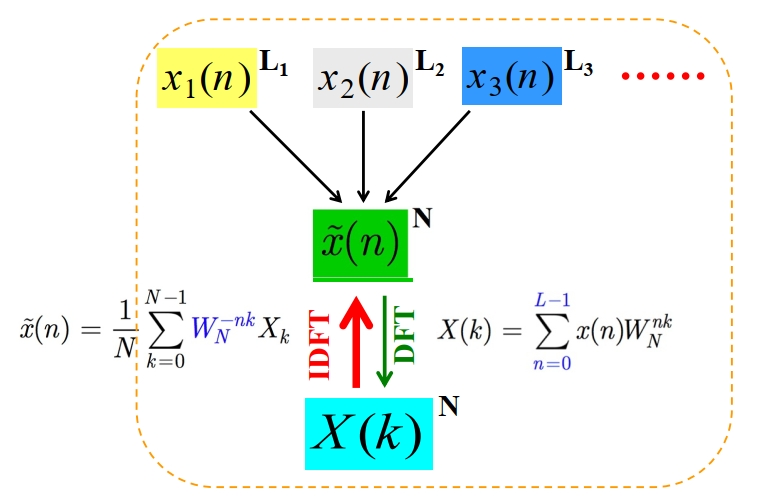
\includegraphics[width = 0.6\textwidth]{chap3/img/wrapped_sequence_relation.png}
        \caption{回绕序列的 DFT 与 IDFT 的关系}
        \label{fig:wrapped_sequence_relation}
    \end{figure}
\end{remark}

\begin{corollary}[$N$ 与 $L$ 的关系]
    DFT、IDFT 中序列的长度 $L$ 与频域采样点个数 $N$ 之间的关系如下:
    \begin{enumerate}[label=(\arabic*)]
        \item $L$ 是待处理的数据长度,不可更改;而 $N$ 则只是数字处理设备中的算法
            参数,由设计人员在使用时设定。
        \item 若 $N > L$,则在数值计算中相当于在序列后面补 $0$,使得 $L = N$。
            虽然这不影响 DFT 结果的正确性,但因补充的 $0$ 使得计算量增大,
            浪费了计算资源。
        \item 若 $N < L$,则可以将序列转为其回绕序列,再进行 DFT。回绕序列的 DFT
            与原序列的 DFT 结果相同。但是回绕序列与原序列的关系是多对一的,
            因此 IDFT 只能得到唯一的一个序列,实际上对应所有序列的回绕序列。
        \item 只有在 $N \ge L$ 时,才能保证 IDFT 的唯一性。
    \end{enumerate}
    结论是,\bd{为了方便计算,通常取 $N = L$}。
\end{corollary}

\subsubsection{离散傅里叶变换的性质}

\begin{property}[DFT 的离散性、周期性]
    设 $x(n)$ 的 DFT 为 $X(k)$,则 $X(k)$ 只能在 $k = 0, 1, \cdots, N - 1$ 处
    取值,且
    \begin{align*}
        X(k) = X(k + N), \quad k = 0, 1, \cdots, N - 1.
    \end{align*}
\end{property}

\begin{property}[DFT 的共轭对称性]
    设 $x(n)$ 为实序列,则
    \begin{align*}
        X^*(N - k) = X(k), \quad k = 0, 1, \cdots, N - 1.
    \end{align*}
\end{property}

\begin{proof}
    由于 $W_N = \mathe^{-2\pi\mathi/N}$,因此
    \begin{align*}
        \left(W_N^{(N - k)n}\right)^* & = \left(\mathe^{-2\pi\mathi n(N-k)/N}\right)^* \\
        & = \mathe^{2\pi\mathi n(k-N)/N} \\
        & = \mathe^{2\pi\mathi kn/N} / \mathe^{2\pi\mathi n} \\
        & = \left(\mathe^{2\pi\mathi/N}\right)^{kn} \\
        & = W_N^{kn}.
    \end{align*}
    由于 $x(n)$ 为实序列,故 $x(n) = x^*(n)$,所以由 DFT 的定义可知
    \begin{align*}
        X^*(N - k) & = \left(\sum_{n = 0}^{N - 1} x(n)W_N^{(N - k)n}\right)^* \\
        & = \sum_{n = 0}^{N - 1} x^*(n)\left(W_N^{(N - k)n}\right)^* \\
        & = \sum_{n = 0}^{N - 1} x(n)W_N^{kn} \\
        & = X(k).
    \end{align*}
    命题得证。
\end{proof}

\begin{property}[DFT 是线性运算]
    设 $x_1(n)$ 和 $x_2(n)$ 的 DFT 分别为 $X_1(k)$ 和 $X_2(k)$,则
    \begin{align*}
        \DFT{a_1x_1(n) + a_2x_2(n)} = a_1X_1(k) + a_2X_2(k).
    \end{align*}
\end{property}

\begin{property}[DFT 的帕斯瓦尔定理]
    设长度为 $L$ 的序列 $x(n)$ 的 DFT 为长度为 $N$ 的频谱 $X(k)$,
    当 $L = N$ 时,有
    \begin{align*}
        \sum_{n = 0}^{N - 1}\|x(n)\|^2 = \frac{1}{N}\sum_{k = 0}^{N - 1}\|X(k)\|^2.
    \end{align*}
\end{property}

\begin{property}[DFT 的奇偶性、虚实性]
    对于奇对称序列、偶对称序列、实序列、虚序列,其 DFT 的性质如下:
    \begin{enumerate}
        \item 奇对称和偶对称序列:
            \begin{itemize}
                \item 奇对称序列的 DFT 是奇对称序列。
                \item 偶对称序列的 DFT 是偶对称序列。
            \end{itemize}
        \item 实序列:
            \begin{itemize}
                \item 实偶序列的 DFT 是实偶序列,实奇序列的 DFT 是虚奇序列。
                \item 实序列的 DFT 的实部是偶序列,虚部是奇序列。
                \item 实序列的模长序列是偶序列,相位序列是奇序列。
            \end{itemize}
        \item 虚序列:
            \begin{itemize}
                \item 虚偶序列的 DFT 是虚偶序列,虚奇序列的 DFT 是实奇序列。
                \item 虚序列的 DFT 的实部是奇序列,虚部是偶序列。
                \item 虚序列的模长序列是偶序列,相位序列是奇序列。
            \end{itemize}
    \end{enumerate}
\end{property}

\begin{property}[DFT 的反褶和共轭的性质]
    设信号 $x(n)$ 的 DFT 为 $X(k)$,则进行反褶和共轭操作后的信号的 DFT 对应关系如下:
    \begin{figure}[H]
        \begin{tabular}
            {c||c|c}
            操作 & 时域 & 频域 \\
            \hline
            反褶 & $x(-n)$ & $X(-k)$ \\
            共轭 & $x^*(n)$ & $X^*(-k)$ \\
            反褶且共轭 & $x^*(-n)$ & $X^*(k)$ \\
        \end{tabular}
    \end{figure}
\end{property}

\begin{property}[DFT 的频域平移特性]
    设长度为 $L$ 的序列 $x(n)$ 的 DFT 为长度为 $N$ 的频谱 $X(k)$,
    当 $L = N$ 时,有
    \begin{align*}
        X(k - k_0) = \DFT{x(n)W_N^{-k_0n}}.
    \end{align*}
\end{property}

\begin{proof}
    由 DFT 的定义可知
    \begin{align*}
        X(k - k_0) & = \sum_{n = 0}^{N - 1}x(n)W_N^{(k - k_0)n} \\
        & = \sum_{n = 0}^{N - 1}\left(x(n)W_N^{-k_0n}\right)W_N^{kn} \\
        & = \DFT{x(n)W_N^{-k_0n}}.
    \end{align*}
    命题得证。
\end{proof}

\begin{property}[DFT 的对称性]
    设长度为 $L$ 的序列 $x(n)$ 的 DFT 为长度为 $N$ 的频谱 $X(k)$,
    当 $L = N$ 时,有
    \begin{align*}
        \DFT{X(n)} = N\rev{x}(-k).
    \end{align*}
\end{property}

\begin{proof}
    由 IDFT 的定义,
    \begin{align*}
        \rev{x}(n) = \frac{1}{N}\sum_{k = 0}^{N - 1}X(k)W_N^{-kn}.
    \end{align*}
    因此
    \begin{align*}
        N\rev{x}(-n) = \sum_{k = 0}^{N - 1}X(k)W_N^{kn}.
    \end{align*}
    将自变量改写为 $n$,即可得到
    \begin{align*}
        N\rev{x}(-k) = \sum_{n = 0}^{N - 1}X(n)W_N^{kn} = \DFT{X(n)}.
    \end{align*}
    命题得证。
\end{proof}

\begin{property}[DFT 的时移特性]
    设长度为 $L$ 的序列 $x(n)$ 的 DFT 为长度为 $N$ 的频谱 $X(k)$,有
    \begin{align*}
        \DFT{x(n - m)} = W_N^{mk}X(k).
    \end{align*}
\end{property}

\begin{proof}
    (方法一)
    DTFT 的时移特性为 $\DTFT{x(n - m)} = \mathe^{-\mathi\omega m}X(\omega)$。
    由于 DFT 可以看做是 DTFT 在离散点上的抽样,故
    \begin{align*}
        \DFT{x(n - m)} & = \left.\left(\mathe^{-\mathi\omega m}X(\omega)\right)\right|_{\omega = \omega_k} \\
        & = \mathe^{-\mathi\omega_k m}X(\omega_k) \\
        & = W_N^{mk}X(k).
    \end{align*}
\end{proof}

\begin{proof}
    (方法二)
    最需要处理的情况是当 $n < m$ 时 $x(n - m)$ 应该如何对应到 $X(k)$。
    可以考虑定义回绕序列
    \begin{align*}
        \rev{x}(n - m) = \begin{cases}
            x(n + N - m), & 0 \le n < m, \\
            x(n - m), & m \le n < N.
        \end{cases}
    \end{align*}
    显然它们的 DFT 是相等的,即
    \begin{align*}
        \DFT{x(n - m)} = \DFT{\rev{x}(n - m)}.
    \end{align*}
    由 DFT 的定义可知
    \begin{align*}
        \DFT{x(n - m)} & = \DFT{\rev{x}(n - m)} \\
        & = \sum_{n = 0}^{m - 1}x(n - m + N)W_N^{kn}
            + \sum_{n = m}^{N - 1}x(n - m)W_N^{kn} \\
        & = \left(\sum_{n = 0}^{m - 1}x(n - m + N)W_N^{(n - m + N)k}
            + \sum_{n = m}^{N - 1}x(n - m)W_N^{(n - m)k}\right)W_N^{mk} \\
        & = \left(\sum_{t = N - m}^{N - 1}x(t)W_N^{tk}
            + \sum_{n = 0}^{N - m - 1}x(t)W_N^{tk}\right)W_N^{mk} \\
        & = \left(\sum_{t = 0}^{N - 1}x(t)W_N^{tk}\right)W_N^{mk} \\
        & = X(k)W_N^{mk}. 
    \end{align*}
    命题得证。
\end{proof}

\begin{property}[DFT 的时域卷积特性]
    设序列 $x_1(n)$ 和 $x_2(n)$ 的 DFT 分别为 $X_1(k)$ 和 $X_2(k)$,
    则
    \begin{align*}
        \DFT{x_1(n) * x_2(n)} = X_1(k)X_2(k),
    \end{align*}
    其中 $x_1(n) * x_2(n) = \sum_{m = -\infty}^{+\infty}x_1(m)x_2(n - m)$。
\end{property}

\begin{property}[DFT 的频域卷积特性]
    设序列 $x_1(n)$ 和 $x_2(n)$ 的 DFT 分别为 $X_1(k)$ 和 $X_2(k)$,
    则
    \begin{align*}
        \DFT{x_1(n)x_2(n)} = \frac{1}{N}X_1(k) \otimes X_2(k),
    \end{align*}
\end{property}

\begin{property}[IDFT 的频域卷积特性]
    设长度为 $L$ 的序列 $x(n)$ 和 $y(n)$ 的 DFT 分别为长度为 $N$ 的序列 $X(k)$ 和 $Y(k)$,
    当 $N = L$ 时,有
    \begin{align*}
        \IDFT{X(k)Y(k)} = \rev{x(n) * y(n)}
        = \sum_{m = 0}^{N - 1}x(m)\rev{y}(n - m)
        = \sum_{m = 0}^{N - 1}x(m)y(n - m)_N = x(n) \otimes y(n).
    \end{align*}
\end{property}

\begin{proof}
    由于 $\IDFT{Z(k)} = \rev{z}(n)$,因此
    \begin{align*}
        \IDFT{X(k)Y(k)} = \rev{x(n) * y(n)}.
    \end{align*}
    将 IDFT 的定义代入,即可得到
    \begin{align*}
        \IDFT{X(k)Y(k)} & = \frac{1}{N}\sum_{k = 0}^{N - 1}X(k)Y(k)W_N^{-nk} \\
        & = \frac{1}{N}\sum_{k = 0}^{N - 1}\sum_{m = 0}^{N - 1}x(m)W_N^{mk}Y(k)W_N^{-nk} \\
        & = \sum_{m = 0}^{N - 1}x(m)\left(\frac{1}{N}\sum_{k = 0}^{N - 1}Y(k)W_N^{mk}W_N^{-nk}\right) \\
        & = \sum_{m = 0}^{N - 1}x(m)\IDFT{Y(k)W_N^{mk}} \\
        & = \sum_{m = 0}^{N - 1}x(m)\rev{y}(n - m).
    \end{align*}
    考虑到回绕一个移位序列相当于循环移位,所以 $\rev{y}(n - m) = y(n - m)_N$,故
    \begin{align*}
        \IDFT{X(k)Y(k)} = \sum_{m = 0}^{N - 1}x(m)y(n - m)_N = x(n) \otimes y(n).
    \end{align*}
    命题得证。
\end{proof}

\begin{remark}
    计算的过程为:反褶、循环移位、相乘、相加。

    $\otimes$ 也是一种卷积,为了突出新卷积与旧卷积的不同,
    同时也为了突出它们之间的相同, 称过去传统的卷积为\bd{线卷积},
    而称此新卷积为序列的圆周卷积,简称\bd{圆卷积}。
\end{remark}

\subsubsection{总结:FT、DTFT、DFT 的性质}

\begin{figure}[H]
    \centering
    \begin{tabular}{c||p{3cm}|p{4cm}|p{4cm}}
        \textbf{ } & \textbf{FT} & \textbf{DTFT} & \textbf{DFT} \\
        \hline
        线性性 & 是 & 是 & 是 \\
        \hline
        时域反褶 & 频域反褶 & 频域反褶 & 频域反褶 \\
        \hline
        时域共轭 & 频域共轭+反褶 & 频域共轭+反褶 & 频域共轭+反褶 \\
        \hline
        对称性 & $\mathcal{F}[F(t)] = 2\pi f(-\omega)$
            & $\DTFT{X(n)} = 2\pi x(-\omega)$
            & $\DFT{X(n)} = N \rev{x}(-k)$ \\
        \hline
        时域平移 & $\mathcal{F}[f(t - t_0)] = \mathe^{-\mathi\omega t_0}F(\omega)$
            & $\DTFT{x(n - n_0)} = \mathe^{-\mathi\omega n_0}X(\omega)$
            & $\DFT{x(n - n_0)} = W_N^{kn_0}X(k)$ \\
        \hline
        频域平移 & $\mathcal{F}[\mathe^{\mathi\omega_0 t}f(t)] = F(\omega - \omega_0)$
            & $\DTFT{\mathe^{\mathi\omega_0 n}x(n)} = X(\omega - \omega_0)$
            & $\DFT{x(n)W_N^{-nk_0}} = X(k - k_0)$ \\
        \hline
        时域卷积 & $\mathcal{F}[f_1(t) * f_2(t)] = F_1(\omega)F_2(\omega)$
            & $\DTFT{x_1(n) * x_2(n)} = X_1(\omega)X_2(\omega)$
            & $\DFT{x_1(n) * x_2(n)} = X_1(k)X_2(k)$ \\
        \hline
        频域卷积 & $\mathcal{F}[f_1(t)f_2(t)] = \frac{1}{2\pi}F_1(\omega) * F_2(\omega)$
            & $\DTFT{x_1(n)x_2(n)} = \frac{1}{2\pi}X_1(\omega) \otimes X_2(\omega)$
            & $\DFT{x_1(n)x_2(n)} = \frac{1}{N}X_1(k) \otimes X_2(k)$ \\
    \end{tabular}
\end{figure}
